\chapter{密度泛函理论}
密度泛函理论(Density Functional Theory, DFT)是目前在材料计算中使用最广泛的一种第一性原理计算方法。与传统的 Hartree-Fock 理论(只考虑了交换能)以及各种考虑进电子关联的 Post-Hartree-Fock 衍生方法相比,DFT 的计算成本相对更低。最早尝试利用密度泛函进行第一性原理计算的是 1927 年 L. Thomas 和 E. Fermi 等人提出的 Thomas-Fermi 模型,这一方法尝试仅使用电子密度来计算量子体系,独立于波函数理论\cite{Fermi1927, Thomas_1927}。为了引入泡利不相容原理,1930 年 P. Dirac 在 Thomas-Fermi 理论中又引入了一项交换能\cite{dirac_1930}。但这一方法给出的电子动能项密度泛函形式过于简单,不能很好地准确描述电子动能项,因此在 Thomas-Fermi-Dirac 理论提出之后,并没有得到广泛应用。后来在此基础上发展起来的密度泛函理论(Density Functional Theory, DFT)使用电子波函数计算动能项,这样就避免了动能项没有精确泛函的问题。同时,密度泛函理论把动能项和电子间库仑相互作用的误差项都放在了能量占比较小的交换关联势中,降低了系统误差。下面逐一介绍作为密度泛函理论出发点的 Thomas-Fermi-Dirac 理论以及密度泛函理论方案的基本原理。
\section{Thomas-Fermi-Dirac 近似及其推广}
Thomas-Fermi 近似认为系统中的电子动能项可以通过将空间划分为小格子,每一个小格子的动能认为是依赖于密度泛函的全同电子气动能,即有
\begin{equation}
    T_{\text{T-F}}=C_{\text{F}}\int\text{d}r^3 \rho^{5/3},\quad C_{\text{F}}\approx 2.871.
\end{equation}
在这一近似下,能量泛函就可以相应地表示为 
\begin{equation}
    E_{\text{T-F}}=C_{\text{F}}\int\text{d}r^3 \rho^{5/3}+\int v(\boldsymbol{r})\rho(\boldsymbol{r})\text{d}r^3+\frac{1}{2}\iint\frac{\rho(\boldsymbol{r}_1)\rho(\boldsymbol{r}_2)}{\left| \boldsymbol{r}_1-\boldsymbol{r}_2 \right|}\text{d}\boldsymbol{r}_1\boldsymbol{r}_2.
\end{equation}
为考虑进电子的交换反对称性质,狄拉克进一步引入交换积分 
\begin{equation}
    K_{ij}=-\int\frac{\phi^*_{k_1}(\vct{r}_1)\phi^*_{k_2}(\vct{r}_2)\phi_{k_1}(\vct{r}_2)\phi_{k_2}(\vct{r}_1)}{\left| \vct{r}_1-\vct{r}_2 \right|}\dd\vct{r}_1\dd\vct{r}_2,
\end{equation}
这样,就得到了 Thomas-Fermi-Dirac 能量泛函的表达式 
\begin{equation}
    \begin{aligned}
        E_{\text{T-F}}=&C_{\text{F}}\int\text{d}r^3 \rho^{5/3}+\int v(\boldsymbol{r})\rho(\boldsymbol{r})\text{d}r^3\\
        &+\frac{1}{2}\iint\frac{\rho(\boldsymbol{r}_1)\rho(\boldsymbol{r}_2)}{\left| \boldsymbol{r}_1-\boldsymbol{r}_2 \right|}\text{d}\boldsymbol{r}_1\dd\boldsymbol{r}_2-C_X\int\dd\rho^{4/3}(\vct{r})\dd\vct{r}.
    \end{aligned}
\end{equation}
这一近似方法使得人们能够有效处理相互作用电子系统。

在这一计算方案中,动能项的密度泛函形式未知,这导致在实际计算中会产生较大的动能项误差。由于没有考虑电子关联,交换能也存在误差。E. Teller 在 1962 年指出,Thomas-Fermi 理论计算得到的任何分子能量都会高于组成这一分子的原子总能,因此这一方案不能用来计算分子成键过程\cite{RevModPhys.34.627}。

密度泛函理论起源于 Thomas-Fermi-Dirac 理论,人们利用 Hohenberg-Kohn 定理将体系的总能量是密度的泛函这一概念加以推广,证明了所有可观测量都是密度的泛函\cite{PhysRev.136.B864}。这一理论使用电子波函数来计算动能项,计算精度高,避免了动能项没有精确泛函的问题,同时把动能项和电子间库仑相互作用的误差都放在交换关联势中,这部分能量比较小。因此相比于 Thomas-Fermi-Dirac 理论,DFT 之后得到了更广泛的应用。下面简单介绍 DFT 的基本原理和计算方案。
\section{基本理论}
1964 年,P. Hohenberg 和 W. Kohn 在非均匀电子气理论的基础上,给出了两条定理:
\begin{theorem}
    在相互作用电子系统中,除了常数项之外,外势场 $V_{\fun{ext}}(\vct{r})$ 可以由基态电子密度 $n_0(\vct{r})$ 唯一确定。
\end{theorem}
\begin{theorem}
    基态总能量泛函 $E[n]$ 可以由基态电子密度 $n_0(\vct{r})$ 和任意给定的外势 $V_{\fun{ext}}(\vct{r})$ 唯一地确定下来。
\end{theorem}
利用反证法(对于定理一:假设同一个基态电子密度 $N_0(\vct{r})$ 可以确定两个不同的外势场;对于定理二:假设有两套基态密度 $n_0(\vct{r})$ 可以确定同一个基态总能量泛函)很容易证明这两条定理\cite{martin_2004},此处不加以赘述。根据这两条定理,基态电子密度就能够唯一地确定体系的哈密顿量(除了常数项),这样体系的全部多体波函数也能够确定下来,这样就得到了密度泛函理论框架中重要的一点,那就是体系的全部物理性质都能够由基态密度 $n_0(\vct{r})$ 唯一地确定下来。

由于两条定理都能被严格证明,证明过程不用取任何近似,因此 DFT 的原始理论本身是精确的。但在实际的物理体系中,只有外势场项的密度泛函表达式是精确已知的,动能项和电子-电子相互作用项并没有精确的密度泛函表达式。这导致原始的 DFT 无法被应用到实际计算中。

为处理这一困难,1965 年 W. Kohn 和 L. Sham 在 DFT 基础上利用一套等效的无相互作用参考电子系统(Kohn-Sham auxiliary system)近似描述多电子系统\cite{PhysRev.140.A1133}。这一方案假定无相互作用的参考电子系统与有相互作用的多电子系统具有相同的基态电子密度,通过求解参考电子系统,就可以得到真实的多电子系统的基态能量和基态电荷密度,是一种近似方案。

在 KS 方程中,参考电子系统的动能泛函是可以求解出来的,库仑相互作用可以使用平均场近似,其他误差都放在交换关联中,其中包含交换能、关联能、电子动能的误差以及库伦势的自相互作用修正。下一小节将具体介绍 Kohn-Sham 框架下的 DFT 基本方程和迭代计算流程。
\section{Kohn-Sham DFT}
Kohn-Sham DFT 的两条基本假设如下。
\begin{itemize}
    \item[(1)] 多电子系统的基态电荷密度可以与一组无相互作用电子系统的基态电荷密度对应起来。人们一般称这一表示方法为“无相互作用 $V$ 可表示性(non-interacting-V-representability)”\cite{ENGLISCH1983253}。这一假设并没有严格的理论证明。
    \item[(2)] 无相互作用的参考电子系统哈密顿量由单电子动能项和等效的局域势场项 $V_{\fun{eff}}^{\sigma}(\vct{r})$ 构成。这样,真实系统的电荷密度就能够写成一些无相互作用波函数密度之和。
\end{itemize}

在这两条基本假设下,实际多电子体系的计算就可以等效地在一个无相互作用粒子系统中展开。参考系统中某一位置处的电荷密度可以表示为
\begin{equation}
    n(\vct{r})=\sum_{\sigma}n(\vct{r},\sigma)=\sum_{\sigma}\sum_{i=1}^{N^\sigma}\left| \psi_i^{\sigma}(\vct{r}) \right|,
\end{equation}
对应的无相互作用系统的动能可以表示为 
\begin{equation}
    T_s=-\frac{1}{2}\sum_{\sigma}\sum_{i=1}^{N^{\sigma}}\llag \psi_i^\sigma \right| \nabla^2 \left| \psi_i^\sigma \rrag = \frac{1}{2}\sum_{\sigma}\sum_{i=1}^{N^\sigma}\int\dd^3 r\left| \nabla \psi_i^\sigma (\vct{r}) \right|,
\end{equation}
然后定义库仑能(也常被称为 Hartree 能)
\begin{equation}
    E_{\fun{Hartree}}[n]=\frac{1}{2}\int\dd^3 r\dd^3 r' \frac{n(\vct{r})n(\vct{r}')}{|\vct{r}-\vct{r}'|},
\end{equation} 
总的 Kohn-Sham 能量泛函表达式就可以表示为 
\begin{equation}
    E_{\fun{KS}}=T_s[n]+\int\dd\vct{r}V_{\fun{ext}}(\vct{r})n(\vct{r})+E_{\fun{Hartree}}[n]+E_{\fun{xc}}[n].
\end{equation}
在这一思想下,波函数的反对称性带来的相互作用被归为交换项;原始体系的关联相互作用统一归为关联项,这两项补充在交换关联能 $E_{\fun{xc}}[n]$ 中。这样,形式上 Kohn-Sham 能量泛函表达式就是严格成立的。

在数值计算求解 KS 方程的过程中,人们往往需要对波函数基底作截断。采用合适的基底可以降低基底的阶数,从而减少计算量。在 WIEN2k 程序\cite{WIEN2k}中使用的是线性缀加平面波(Linearized Augmented plane wave, LAPW)基底,这一方案在靠近原子核附近划定一个范围,称为 Muffin-tin 球,球内使用球谐函数展开,球外使用平面波展开,这样就能够较好地同时描述原子核附近剧烈变化的波函数和远离原子核处平缓的波函数\cite{lapw}。LAPW 是目前计算晶体电子结构最精确的方案之一。

如果体系的交换关联泛函已知,那么基态能和多电子系统的电荷密度就能够通过求解 Kohn-Sham 单电子方程得到。对于大部分交换关联泛函形式未知的实际系统,人们给出各种近似方案来表示这一项,这也使得计算多电子系统变得可能。事实上,密度泛函理论的一个重要方向就是不断发展更准确的交换关联形式,使计算结果更可靠。

在 KS 方程中,最早使用的交换关联泛函采用的是局域密度近似(Local Density Approximation, LDA),这一方案的思想仍然基于均匀电子气,认为交换关联泛函的每一点取值只和这一点的电荷密度有关。考虑到交换能和关联能的物理含义不同,需要分开处理,有
\begin{equation}
    E_{\fun{xc}}[n]=E_{\fun{x}}[n]+E_{\fun{c}}[n].
\end{equation}
在 LDA 近似下,交换项和关联项可以分别表示为 
\begin{equation}
    E_{\fun{x}}^{\fun{LDA}}[n]=\int \dd^3 r\ n(\vct{r})\epsilon_{\fun{x}}[n(\vct{r})],\quad E_{\fun{c}}^{\fun{LDA}}[n]=\int \dd^3 r\ n(\vct{r})\epsilon_{\fun{c}}[n(\vct{r})],
\end{equation}
其中 $\epsilon_{\fun{x}}[n(\vct{r})]$ 和 $\epsilon_{\fun{c}}[n(\vct{r})]$ 是密度为 $n$ 的电子气中单个电子对应的交换能和关联能,交换能可以严格推导得到,但关联能没有严格的解析表达式。1980 年, D. Ceperley 和 B. Alder 等人利用量子蒙特卡洛方法得到了较为精确的关联能数值结果\cite{PhysRevLett.45.566},后来人们对这一数值结果进行参数化,得到了两种关联能量密度的具体表达式\cite{PhysRevB.23.5048,PhysRevB.45.13244}。

但是对于电子势场在空间中变化剧烈的体系,LDA 近似就不再适用。在此基础上,人们考虑添加一项密度梯度修正项,这样就得到了各种广义梯度近似(Generalized Gradient Approximation, GGA)的交换关联泛函,比如在实际计算中常使用的 B88\cite{B88},PW91\cite{PW91},PBE\cite{PBE} 泛函等。然而 GGA 近似仍然是一个局域泛函,无法考虑长程关联,所以这种近似方案仍然不能很好地处理强关联电子系统。
\begin{figure}[H]
    \vspace{13pt} % 调整图片与上文的垂直距离
    \centering
    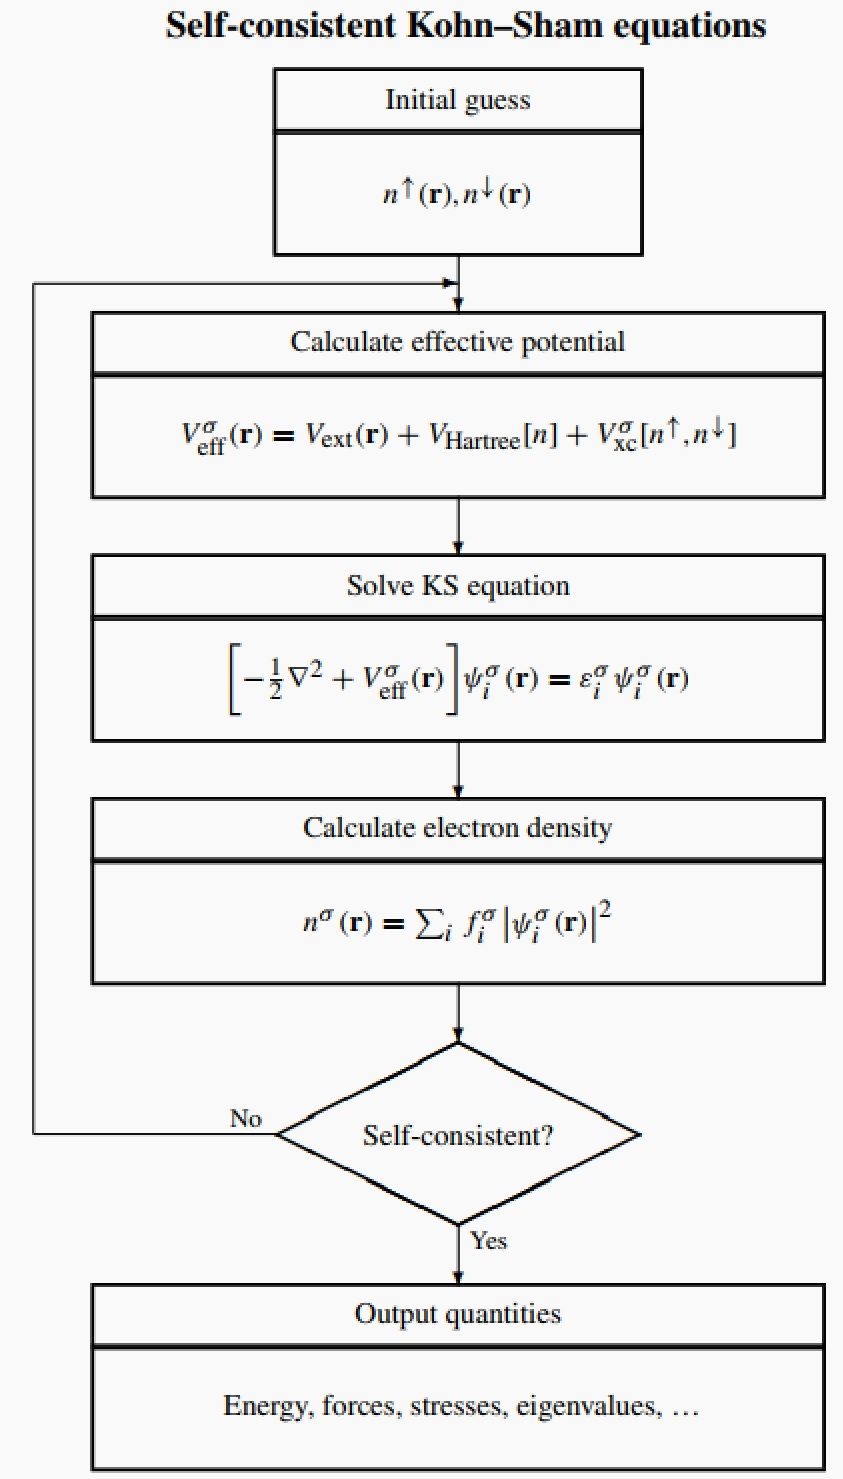
\includegraphics[width=3.5in]{Img/ks-scf.png}
    \caption{KS-DFT 自洽计算流程示意图\cite{martin_2004}。}
    \label{KS-scf} 
\end{figure}
DFT 自洽计算的一般流程如图 \ref{KS-scf} 所示,首先根据初始输入的晶格信息等参数计算出初始电荷密度 $n^{\ua}(\vct{r})$ 和 $n^\da(\vct{r})$,利用这一电荷密度计算出 DFT 的等效外势场 $V_{\fun{eff}}^{\sigma}(\vct{r})$(对应 WIEN2k 的 lapw0 程序),接着利用这一势场求解单电子近似下的 KS 方程(对应 lapw1 程序)得到本征值和本征波矢,再利用这些计算结果得到体系的费米能和新的电荷密度(对应程序 lapw2),如果新旧电荷密度不收敛,则使用 mixer 程序混合新旧电荷密度重复上述步骤,如果电荷收敛,则完成自洽计算,可以进一步使用计算得到的电荷密度分析各种实际物理量。

在强关联电子体系的计算中,密度泛函理论会出现较大问题。例如 3$d$ 电子的过渡金属氧化物、4$f$ 电子的稀土氧化物、5$f$ 电子的锕系元素氧化物中,电子关联带来的效应不能被忽略。一个 DFT 失效的典型问题是对 Mott 绝缘体的预测。DFT 电子结构计算通常会给出金属基态,但实验结果是带隙较宽的绝缘体。这是因为 Mott 绝缘体中通常具有部分填充的 $d$ 电子壳层,其中存在很强的库仑相互作用。如果库仑相互作用 $U$ 大于带宽 $W$,电子将趋于局域化,因此体系会出现由关联效应导致的绝缘性质。密度泛函理论这种单电子近似方法不能很好地描述这种关联性质。一些简单的修正方法能够一定程度上改进这一缺陷。最常用的方法是在电子的 $d$ 或 $f$ 轨道的势能项中引入库仑相互作用项,这被称为 LDA+$U$ 方法。下面简单介绍一下这一方法的基本思路。
\section{LDA+$U$}
在 LDA+$U$ 方法中,相互作用项定义为 
\begin{equation}
    H_U\equiv \sum_{\sigma\sigma'}\sum_{mm''m'm'''}U_{mm''m'm'''}a_{m\sigma}^\dg a_{m''\sigma'}^\dg a_{m'''\sigma'}^{ }a_{m'\sigma}^{ },
\end{equation}
其中 
\begin{equation}
    U_{mm''m'm'''}\equiv \frac{1}{2}\llag mm''\left| V_{ee} \right| m'm''' \rrag.
\end{equation}
如果将体系的电荷密度划分为弱关联和强关联两部分,弱关联部分用 $\rho$ 表示,强关联部分用 $n$ 表示,可以将能量泛函写成下面的形式:
\begin{equation}
    E^{\fun{LDA}+U}[\rho,n]=E^{\fun{LDA}}[\rho]+E^{U}[n]-E_{\fun{dc}}[n],
\end{equation}
其中 $E_{\fun{dc}}$ 称为双计数项,用于扣除前两项的重叠部分。双计数项目前并没有严格的数学形式,针对不同体系人们采用了不同的双计数项方案,例如在弱关联和半导体系统中适用的 AMF 方案\cite{PhysRevB.44.943,PhysRevB.49.14211}、在接近整数占据的体系中适用的 FLL 方案\cite{PhysRevB.48.16929}、AMF 和 FLL 的插值混合方法\cite{PhysRevB.67.153106}、以及能够对自相互作用项更好修正的方案\cite{PhysRevB.76.033102}等。

然而 LDA+$U$ 方法实际上引入的是静态的相互作用,这一般会高估相互作用效应,并且在平均场意义下无法得到强关联体系的近藤物理。为了克服这一局限性,人们需要在平均场理论的基础上进一步考虑动态效应的修正。动力学平均场理论就是这样一种超越平均场理论的方案,通过将密度泛函理论与动力学平均场理论结合,人们可以在实际材料中计算得到近藤物理的相关性质。下面简要介绍动力学平均场理论的主要方法,以及将密度泛函理论与动力学平均场理论结合的计算方案。
